\chapter{\ChapterTitleProjectVision}
\label{sec:cel-wizja}

%%%

\section{Charakterystyka problemu}

Gry karciane, takie jak brydż, cieszą się dużą popularnością na całym świecie.
Jednakże, wiele osób ma trudności w~znalezieniu odpowiednich partnerów do gry,
szczególnie w przypadku osób początkujących, które nie posiadają jeszcze
szerokiego kręgu znajomych zainteresowanych tą grą. W~takiej sytuacji, osoby
chcące nauczyć się gry w~brydża lub doskonalić swoje umiejętności, często
zniechęcają się do dalszego uczestnictwa w~rozgrywkach.

Ponadto, brydż jest grą wymagającą nie tylko umiejętności logicznego myślenia
i~strategii, ale także zdolności do skutecznej komunikacji i~współpracy
z~partnerem. Wielu początkujących graczy nie jest w~stanie zagrać pełnej
i~satysfakcjonującej gry, gdyż nie posiadają odpowiedniego doświadczenia
i~umiejętności. Dodatkowo, niektórzy mogą nie być w stanie znaleźć
partnera, który miałby taki sam styl gry lub nie rozumieją strategii,
które chcieliby zastosować.

W~związku z~powyższymi problemami, zidentyfikowano potrzebę opracowania
aplikacji do gry w brydża, która umożliwiłaby grę z~wirtualnym asystentem
na poziomie umiejętności dostosowanym do użytkownika, zapewniającym satysfakcjonującą
rozgrywkę oraz możliwość nauki i~doskonalenia umiejętności gry w~brydża.

%%%

\section{Motywacja projektu}

\begin{figure}
    \centering
    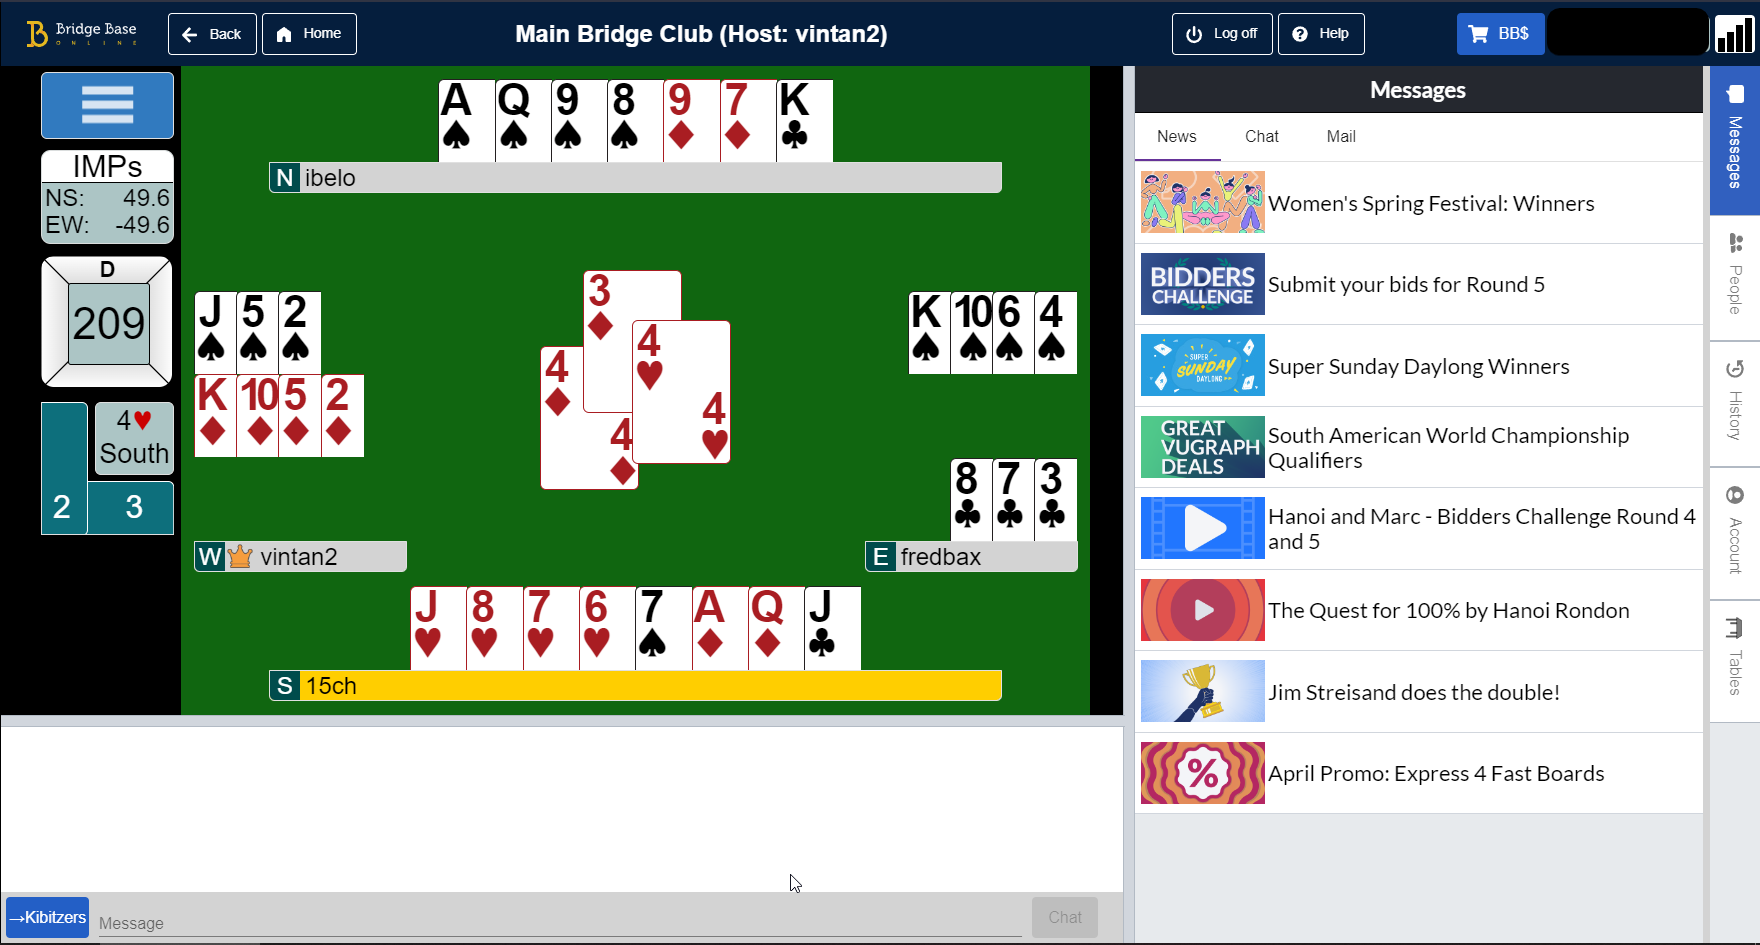
\includegraphics[width=0.9\textwidth]{img/brydz-platformy/bridgebase.png}
    \caption{Rozgrywka brydża na platformie Bridge Base}
    \label{fig:bridge-base}
\end{figure}

\begin{figure}
    \centering
    \subfloat[Główny ekran rozgrywki]{
        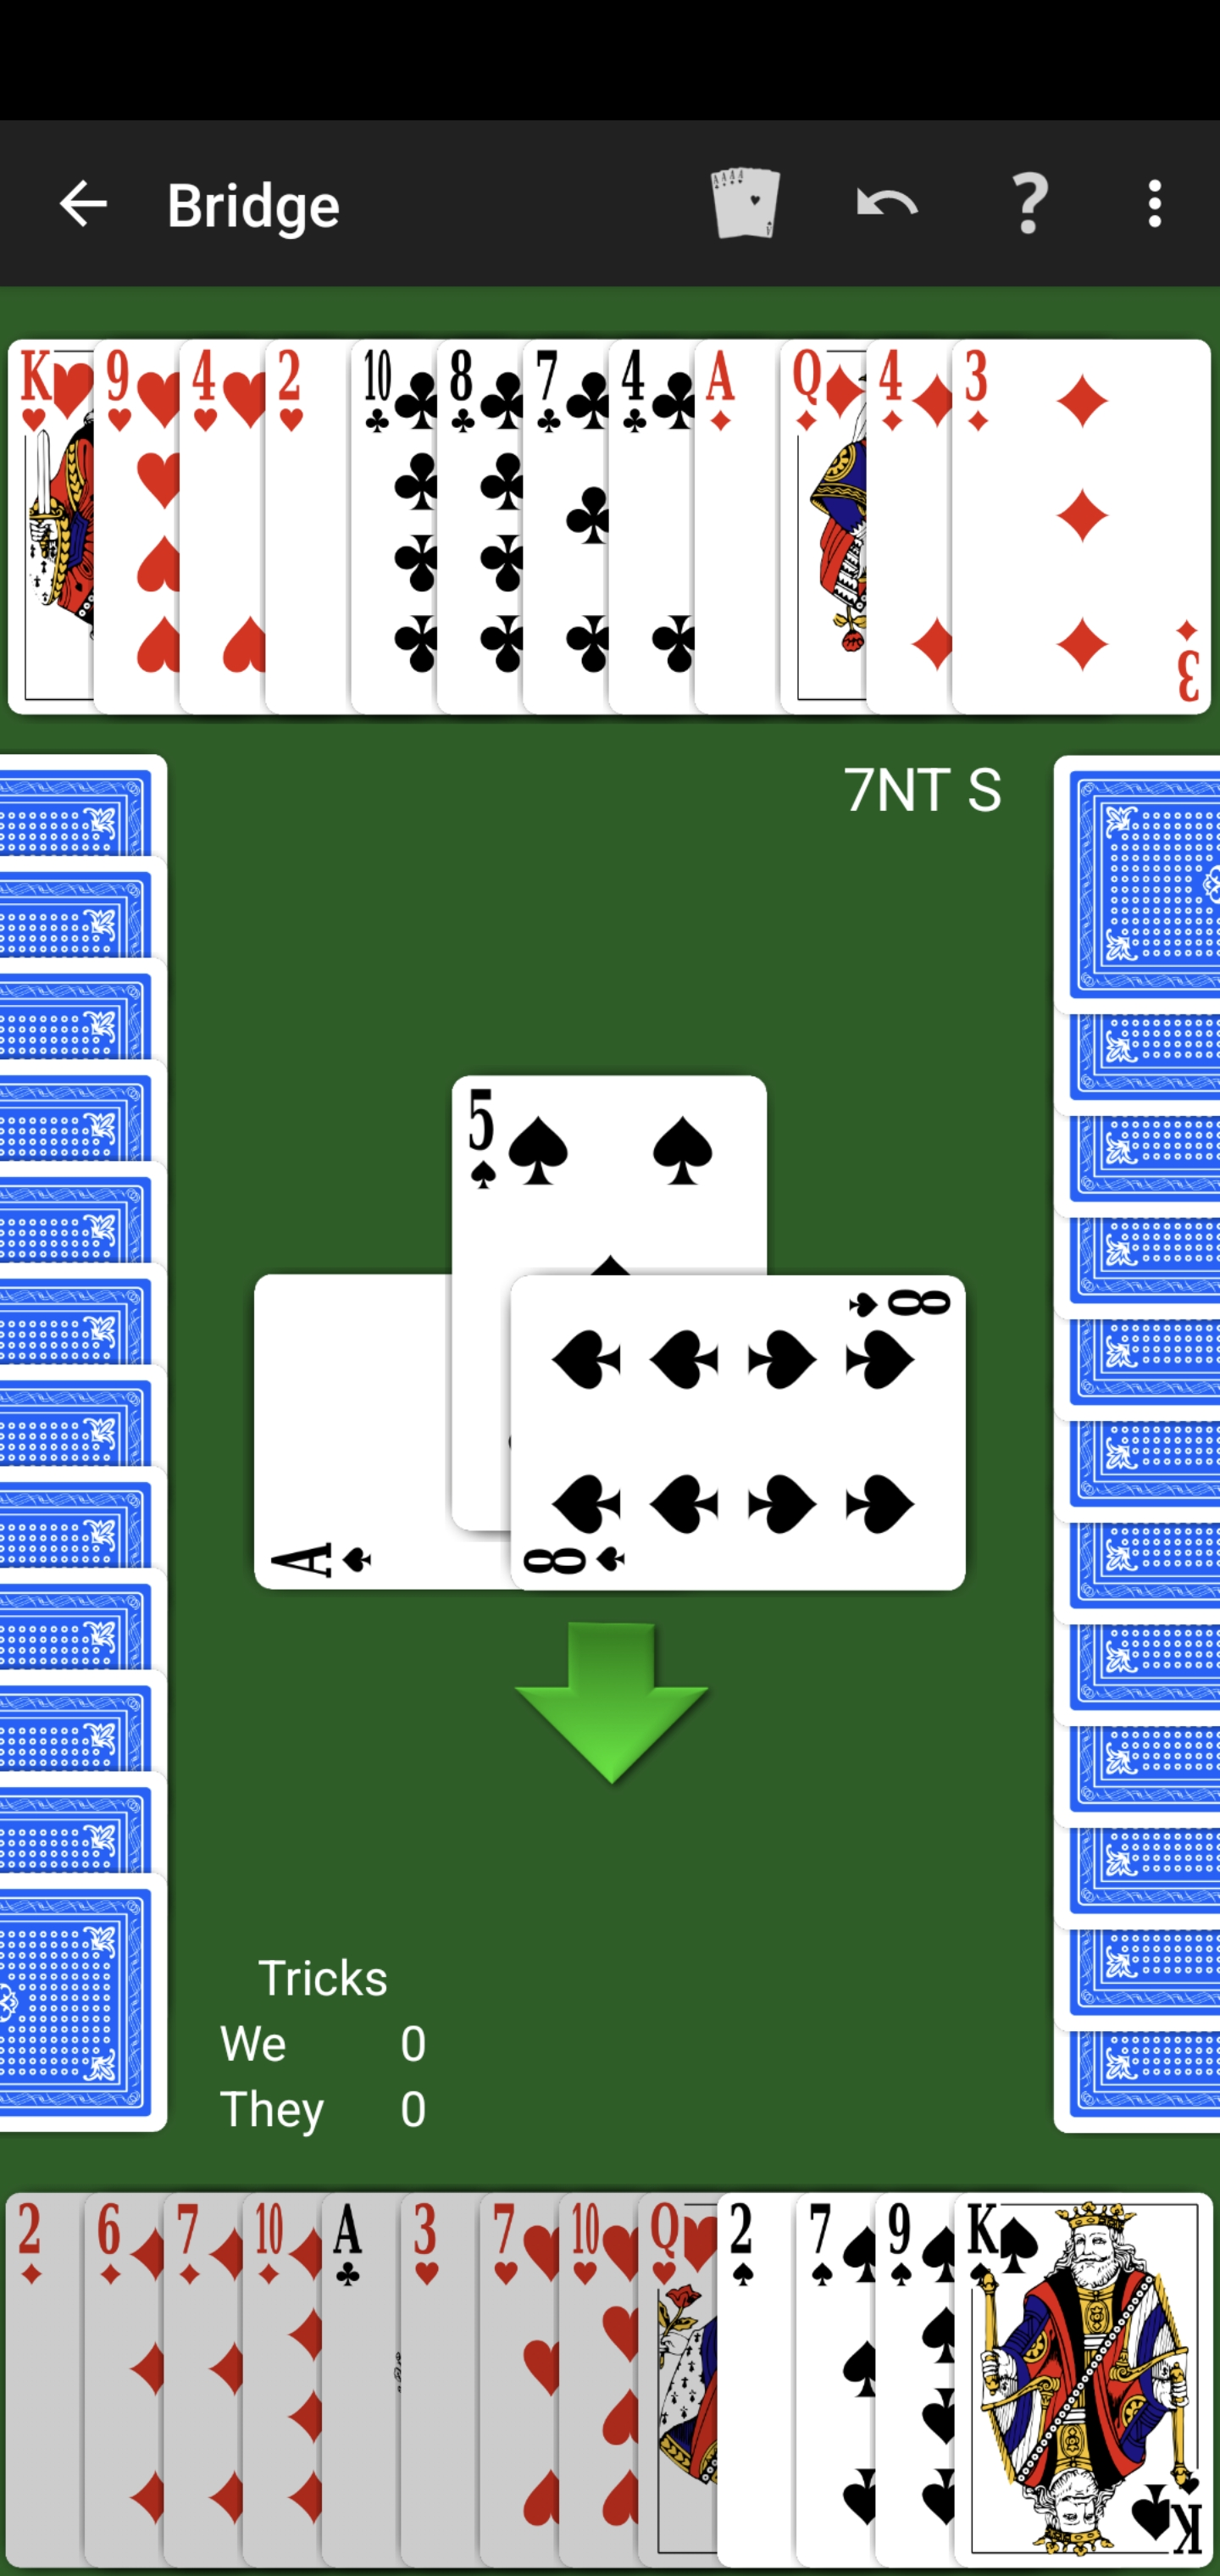
\includegraphics[width=.4\textwidth]{img/brydz-platformy/neuralplay1.jpg}
        \label{fig:neural-play-1}
    }%
    \hspace*{0.5cm}
    \subfloat[Historia bieżącej rozgrywki]{
        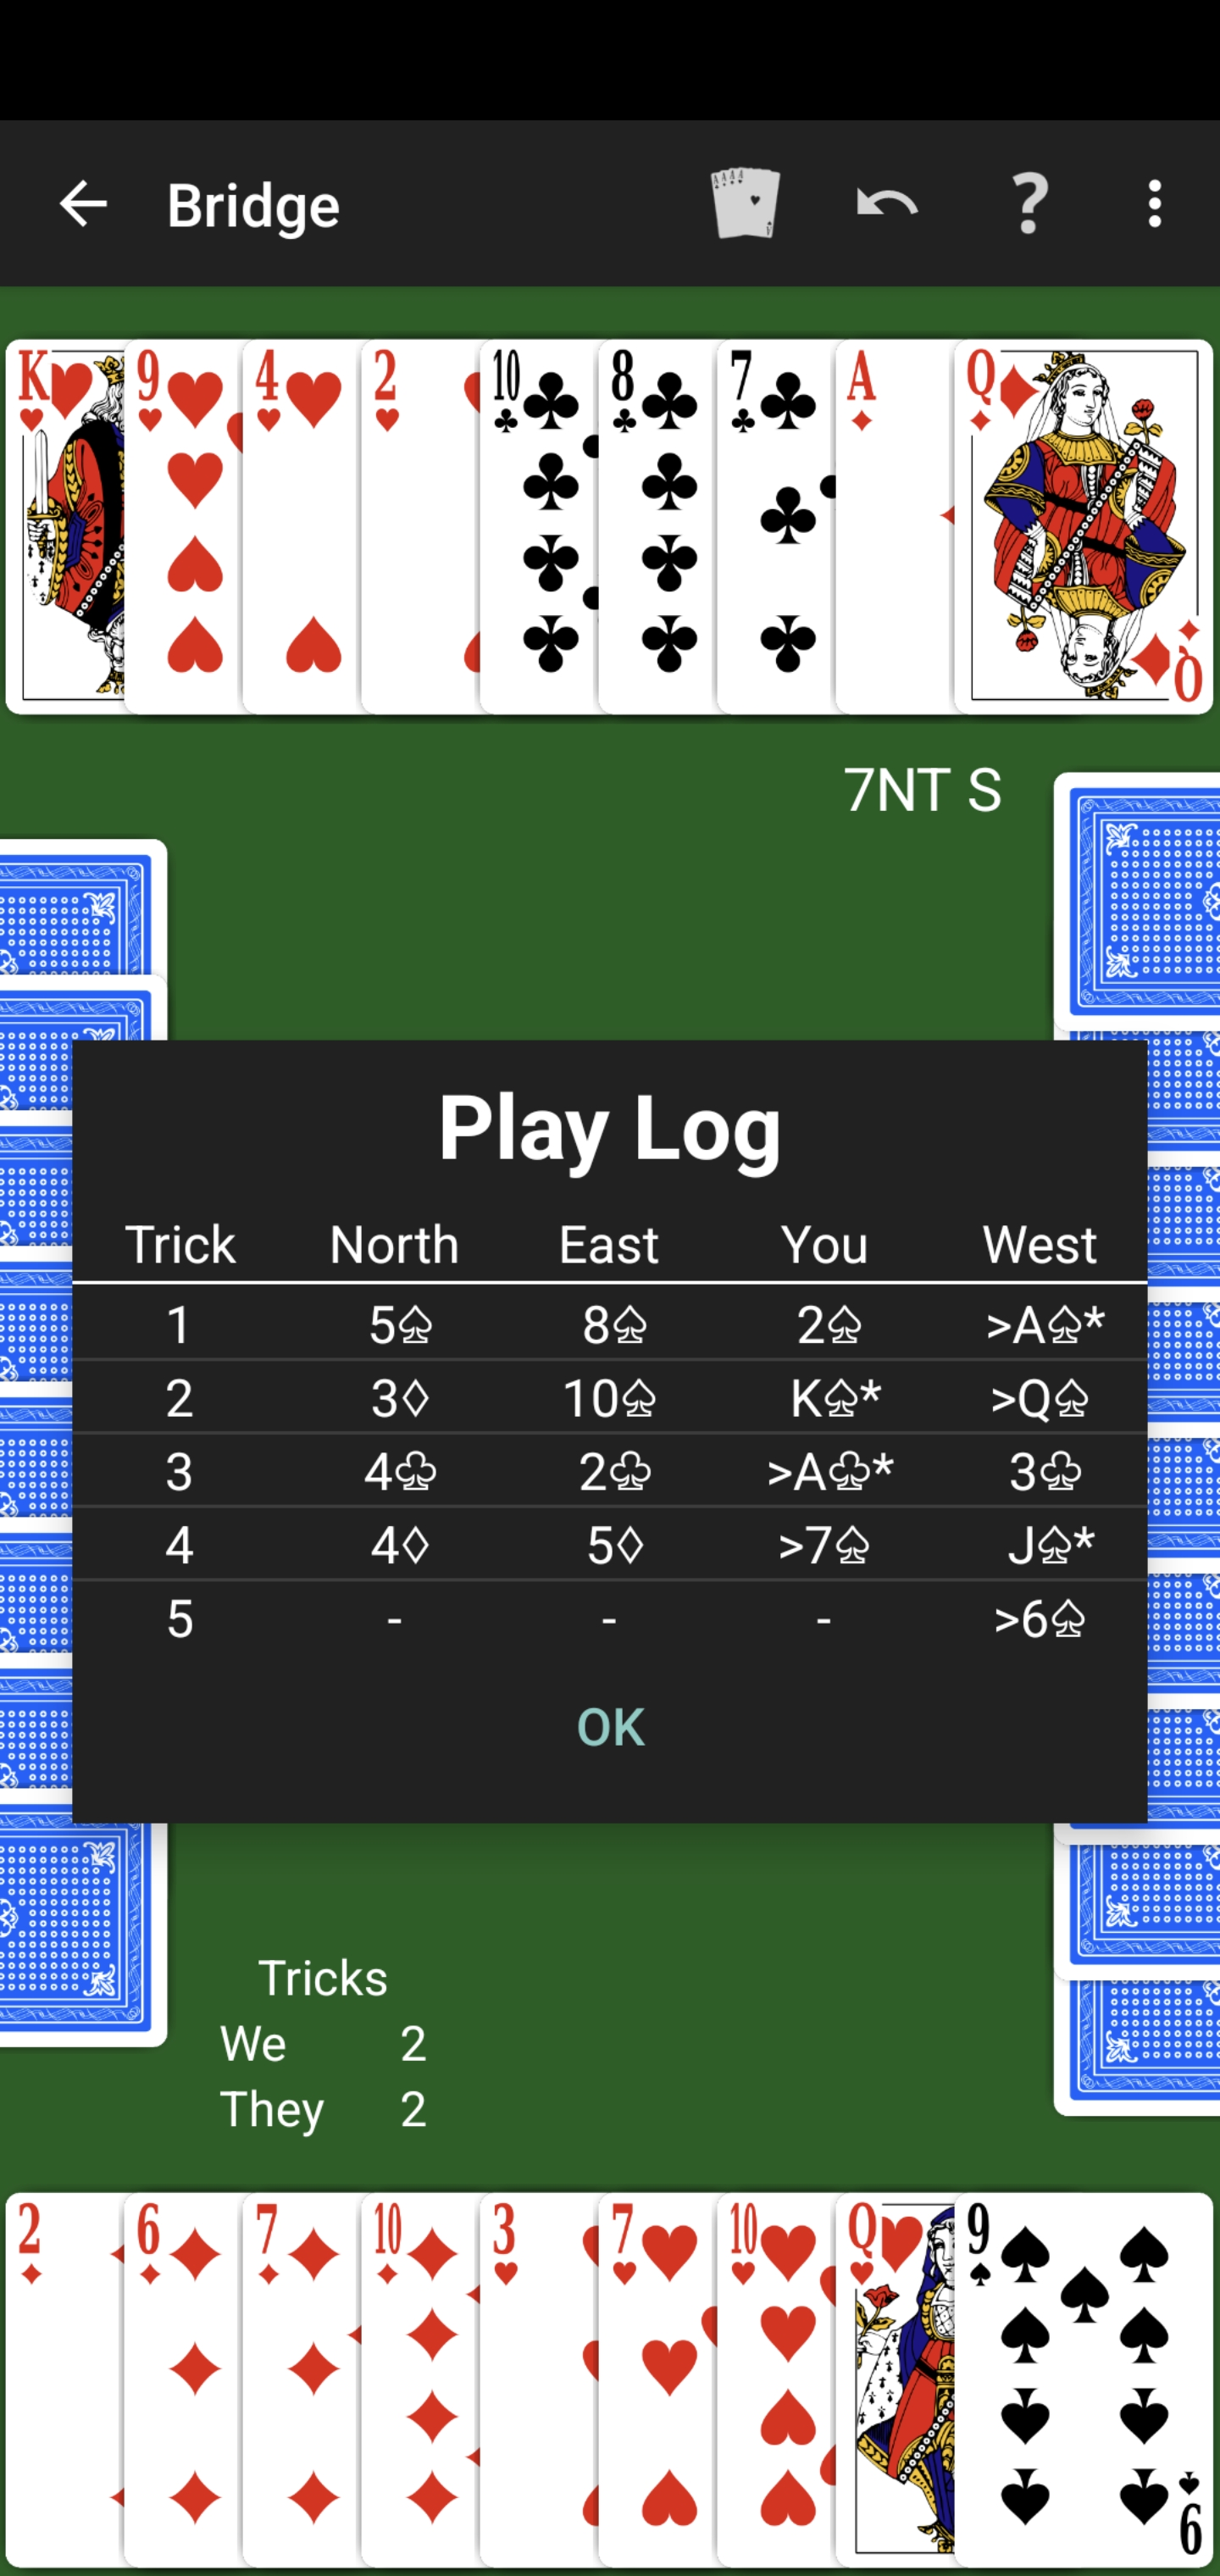
\includegraphics[width=.4\textwidth]{img/brydz-platformy/neuralplay2.jpg}
        \label{fig:neural-play-2}
    }%
    \caption{Rozgrywka brydża w aplikacji Bridge by NeuralPlay}
    \label{fig:neural-play}
\end{figure}

Wirtualny asystent może stanowić rozwiązanie dla tych problemów. Poprzez
zintegrowanie sztucznej inteligencji z~brydżem, aplikacja będzie w~stanie
zapewnić użytkownikom nie tylko wskazówki dotyczące gry, ale także możliwość
rozgrywania partii z~wirtualnym partnerem, który będzie reagował na decyzje
gracza i~pomagał mu w~rozwijaniu jego umiejętności.

Dzięki temu projektowi, użytkownicy będą mieli możliwość łatwiejszego i~bardziej
efektywnego nauczania się gry w~brydża, oraz lepszego dostępu do partnerów
do gry, co pozwoli na bardziej intensywny i~satysfakcjonujący rozwój ich
umiejętności i~pasji. Umożliwi użytkownikom naukę i~doskonalenie umiejętności
w~grze z~wirtualnym partnerem, który byłby w~stanie udzielać cennych
wskazówek i~pomocy w~trakcie gry.
\newline

Obecnie na rynku istnieje kilka analogicznych rozwiązań, jak na przykład
aplikacje internetowe Funbridge \cite{funbridge}, Bridge Base \cite{bridgebase},
BridgeAce+ \cite{bridgeace} oraz mobilna wersja Bridge by NeuralPlay
\cite{neuralplay}. W~przypadku BridgeAce+, użytkownik może korzystać wyłącznie
z~opcji nauki brydża w pojedynkę, gdzie partnerem i~przeciwnikami są boty
wykorzystujące sztuczną inteligencję. Natomiast Funbridge pozwala graczom
rywalizować ze sobą przez Internet oraz uczyć się grając z~botem oraz
przechodząc kursy. Po zakończeniu rozgrywki, użytkownik może przeanalizować
swoje błędy, jednak dostęp do tej opcji wymaga wykupienia konta premium.
Bridge Base oferuje wiele trybów gry, zarówno przeciwko botom jak i~innym
użytkownikom, jednak jego minus stanowi mało intuicyjny interfejs graficzny
Rys.~\ref{fig:bridge-base}. Aplikacja NeuralPlay oferuje pełną rozgrywkę w~brydża
z~wykorzystaniem zaprojektowanego AI, które zna wybrane metody licytowania.
Niestety, nawet rozgrywka przeciwko najtrudniejszemu poziomowi sztucznej
inteligencji, może być wygrana przez osobę mało doświadczoną.
\newline

Jak można zauważyć, istnieją już dostępne aplikacje umożliwiające naukę
i~grę w brydża, jednak mają one istotne wady. Brakuje rozwiązania, które
byłoby dostępne bez konieczności ponoszenia kosztów, umożliwiało naukę
i~rywalizację z~innymi użytkownikami oraz posiadało intuicyjny i~przyjazny
interfejs graficzny. Naszym celem jest połączenie większości tych funkcji
w~naszej własnej aplikacji.



\FloatBarrier

\section{Wizja produktu}

Produkt będzie aplikacją webową umożliwiająca grę w~brydża,
bez konieczności posiadania znajomych do gry.
Partnera lub przeciwnika będzie mógł zastąpić wirtualny asystent.
Jego zadaniem jest zapewnienie odpowiedniego
dla użytkownika towarzysza, którego poziom jest zależny od wybranej
preferencji. Użytkownicy będą mogli dostosować trudność, aby asystent osiągnął
planowane przez nich cele, takie jak nauka, rozgrywka na podobnym poziomie
lub zostać wyzwaniem dla doświadczonych zawodników.

Aplikacja będzie również umożliwiała grę w~brydża z~udziałem jednego lub więcej użytkowników,
którzy będą mogli połączyć się przez Internet, dzięki centralnemu serwerowi.
Zamierzane jest zaprojektowanie jej w~taki sposób, aby była intuicyjna i~łatwa
w~obsłudze dla wszystkich użytkowników, zarówno początkujących, jak
i~doświadczonych.

%%%

\section{Stos technologiczny}

Aplikacja internetowa zostanie napisana w~frameworku React \cite{React}.
Zdecydowaliśmy się na ten wybór, ze względu na dużą popularność tej
technologii. W~2022 roku serwis Stack Overflow \cite{StackOverflow} przeprowadził ankietę dotyczącą między innymi wykorzystywanych technologii
webowych \cite{React-stack}. Aż 42.62\% respondentów wybrało React,
zajmując 2 miejsce w~rankingu. Jako że wykorzystuje on język Javascript,
który według wspomnianej ankiety jest najpopularniejszym językiem programowania,
dostępna jest olbrzymia baza bibliotek i~sprawdzonych rozwiązań. Za wizualną
część projektu będzie odpowiedzialny framework Tailwind CSS \cite{Tailwind}.
Oferuje on gotowe klasy CSS, które pozwalają na szybkie tworzenie responsywnych
i~estetycznych interfejsów. Część serwerowa obsługująca sesje gier zostanie
napisana w~języku Python \cite{Python} za pomocą biblioteki FastAPI
\cite{FastAPI}. Funkcjonalność związana z~obsługą użytkowników i~gromadzenia
danych będzie wykorzystywała usługę Google Firebase \cite{Firebase}.

Wirtualny asystent zostanie zrealizowany jako osobna biblioteka udostępniająca
własne API. Backend obsługujący sesje gier, po dołączeniu biblioteki asystenta,
będzie mógł wysłać do API asystenta aktualny stan gry, aby otrzymać
odpowiedź zawierającą analizę tego stanu, między innymi
prawdopodobieństwo wygrania każdej z~par graczy oraz listę
najlepszych ruchów, jakie mogą być wykonane przez następnego gracza.

Na podstawie wstępnych badań, wybrane zostało 5~algorytmów AI,
które będą rozważane do zastosowania w~projekcie asystenta.
W~kolejności od najbardziej złożonego do
najprostszego w implementacji są to:
\begin{enumerate}
    \item \textbf{Algorytm Regularized Nash Dynamics \cite{doi:10.1126/science.add4679}}\\
          Algorytm oparty na teorii gier, który wykorzystuje sieć neuronową do
          predykcji najlepszego ruchu. Istnieje dowód formalny, że algorytm
          zbiega do równowagi Nasha, czyli optymalnej strategii.

    \item \textbf{Algorytm AlphaZero \cite{AlphaZeroPaper} połączony z algorytmem IS-MCTS \cite{6203567}}\\
          Algorytm AlphaZero jest wariantem algorytmu Monte Carlo Tree Search,
          który wykorzystuje sieć neuronową do oceny stanu gry.
          Algorytm Information Set MCTS (IS-MCTS) jest modyfikacją algorytmu MCTS, która pozwala na
          przeszukiwanie drzewa stanów gry o~niepełnej informacji.
          Możliwe jest połączenie tych dwóch algorytmów, aby uzyskać
          Information Set AlphaZero.

    \item \textbf{Implementacja algorytmu IS-MCTS z biblioteki OpenSpiel \cite{LanctotEtAl2019OpenSpiel}}\\
          Biblioteka OpenSpiel zawiera implementację algorytmu IS-MCTS,
          który może być wykorzystany do gry w~brydża.

    \item \textbf{Program AI do brydża GIB \cite{Ginsberg1999GIBST}}\\
          GIB jest jednym ze starszych programów AI do brydża. Możliwe jest
          jego bezpośrednie wykorzystanie w~projekcie.

    \item \textbf{Algorytm Pure Monte Carlo Tree Search \cite{pmcts}}\\
          Algorytm równoważny MCTS dla maksymalnej głębokości drzewa równej 1.
\end{enumerate}


%%%

\section{Analiza zagrożeń}
\label{sec:analiza_zagrozen}

Gra w~brydża jest jedną z~najtrudniejszych gier strategicznych na świecie.
Do tej pory nie powstał żaden system AI grający na mistrzowskim poziomie
uwzględniający pełną wersję gry z~licytacją \cite{Bethe2021AdvancesIC}.
Implementacja gracza AI o~wystarczająco wysokim poziomie umiejętności może
być znacznym wyzwaniem. W~literaturze zostało opisane wiele metod AI do brydża
\cite{Zhang2019DesignAD,Zhang2022TheSO,Zhang2022AIEB,Ginsberg1999GIBST}
co sugeruje, że jest to temat dalej otwarty i~ciągle rozwijany.
Przedstawiliśmy 5~różnych możliwości implementacji AI.
W~razie problemów z~implementacją jednej z~nich, pozostałe
zostaną wykorzystane jako plany awaryjne.

Ważnym elementem każdej gry online jest niezawodność systemu
backend oraz jego odporność na awarie.
Aplikacja musi być również odporna na problemy sieciowe.
Platforma Firebase zapewnia nam mechanizmy zabezpieczające
przed problemami po stronie klienta, połączenia internetowego
oraz samego backendu Firebase, który jest redundantnie
rozproszony po całym świecie.
Samo hostowanie strony internetowej zostanie zrealizowane
usługą Firebase Hosting, która również zapewnia wysoką
niezawodność.
Bezpieczeństwo aplikacji będzie zarządzane za pomocą
usługi Firebase Authentication.

Powyżej wymienione usługi są dostępne w darmowym planie.
Podczas pracy nad projektem może dojść do sytuacji, że
zostaną one przekształcone w~plan płatny.
Jeśli dostępne platformy chmurowe staną się niedostępne,
zastosowany zostanie własny serwer działający
w~oparciu o~komputer osobisty lub mikrokomputer, np. Raspberry Pi \cite{RPi}.

% needs latex magic
\begin{table}[h]
  \centering
  \begin{tabularx}{\textwidth}{|p{5.5cm}|Y|Y|}
    \hline
    \textbf{Zagrożenie}                                    & \textbf{Prawdopodobieństwo wystąpienia} & \textbf{Zagrożenie dla projektu} \tabularnewline[0.2cm]
    \hline
    Problemy w implementacji AI                            & Wysokie                                 & Średnie (podano plany awaryjne)  \tabularnewline[0.2cm]
    Nie osiągniecie poziomu mistrzowskiego przez asystenta & Wysokie                                 & Niskie                           \tabularnewline[0.3cm]
    Niska niezawodność produktu                            & Niskie                                  & Średnie                          \tabularnewline[0.1cm]
    Niska niezawodność produktu                            & Niskie                                  & Średnie                          \tabularnewline[0.1cm]
    \hline
  \end{tabularx}
  \caption{Analiza zagrożeń}
  \label{tab:zagrozenia}
\end{table}

%%%

\newpage

\section{Szkic aplikacji}

Zostały przygotowane szkice interfejsu aplikacji
(Rys.~\ref{fig:figma_login}--\ref{fig:figma_game}).

\begin{figure}[h!]
    \centering
    \subfloat[Ekran logowania]{
        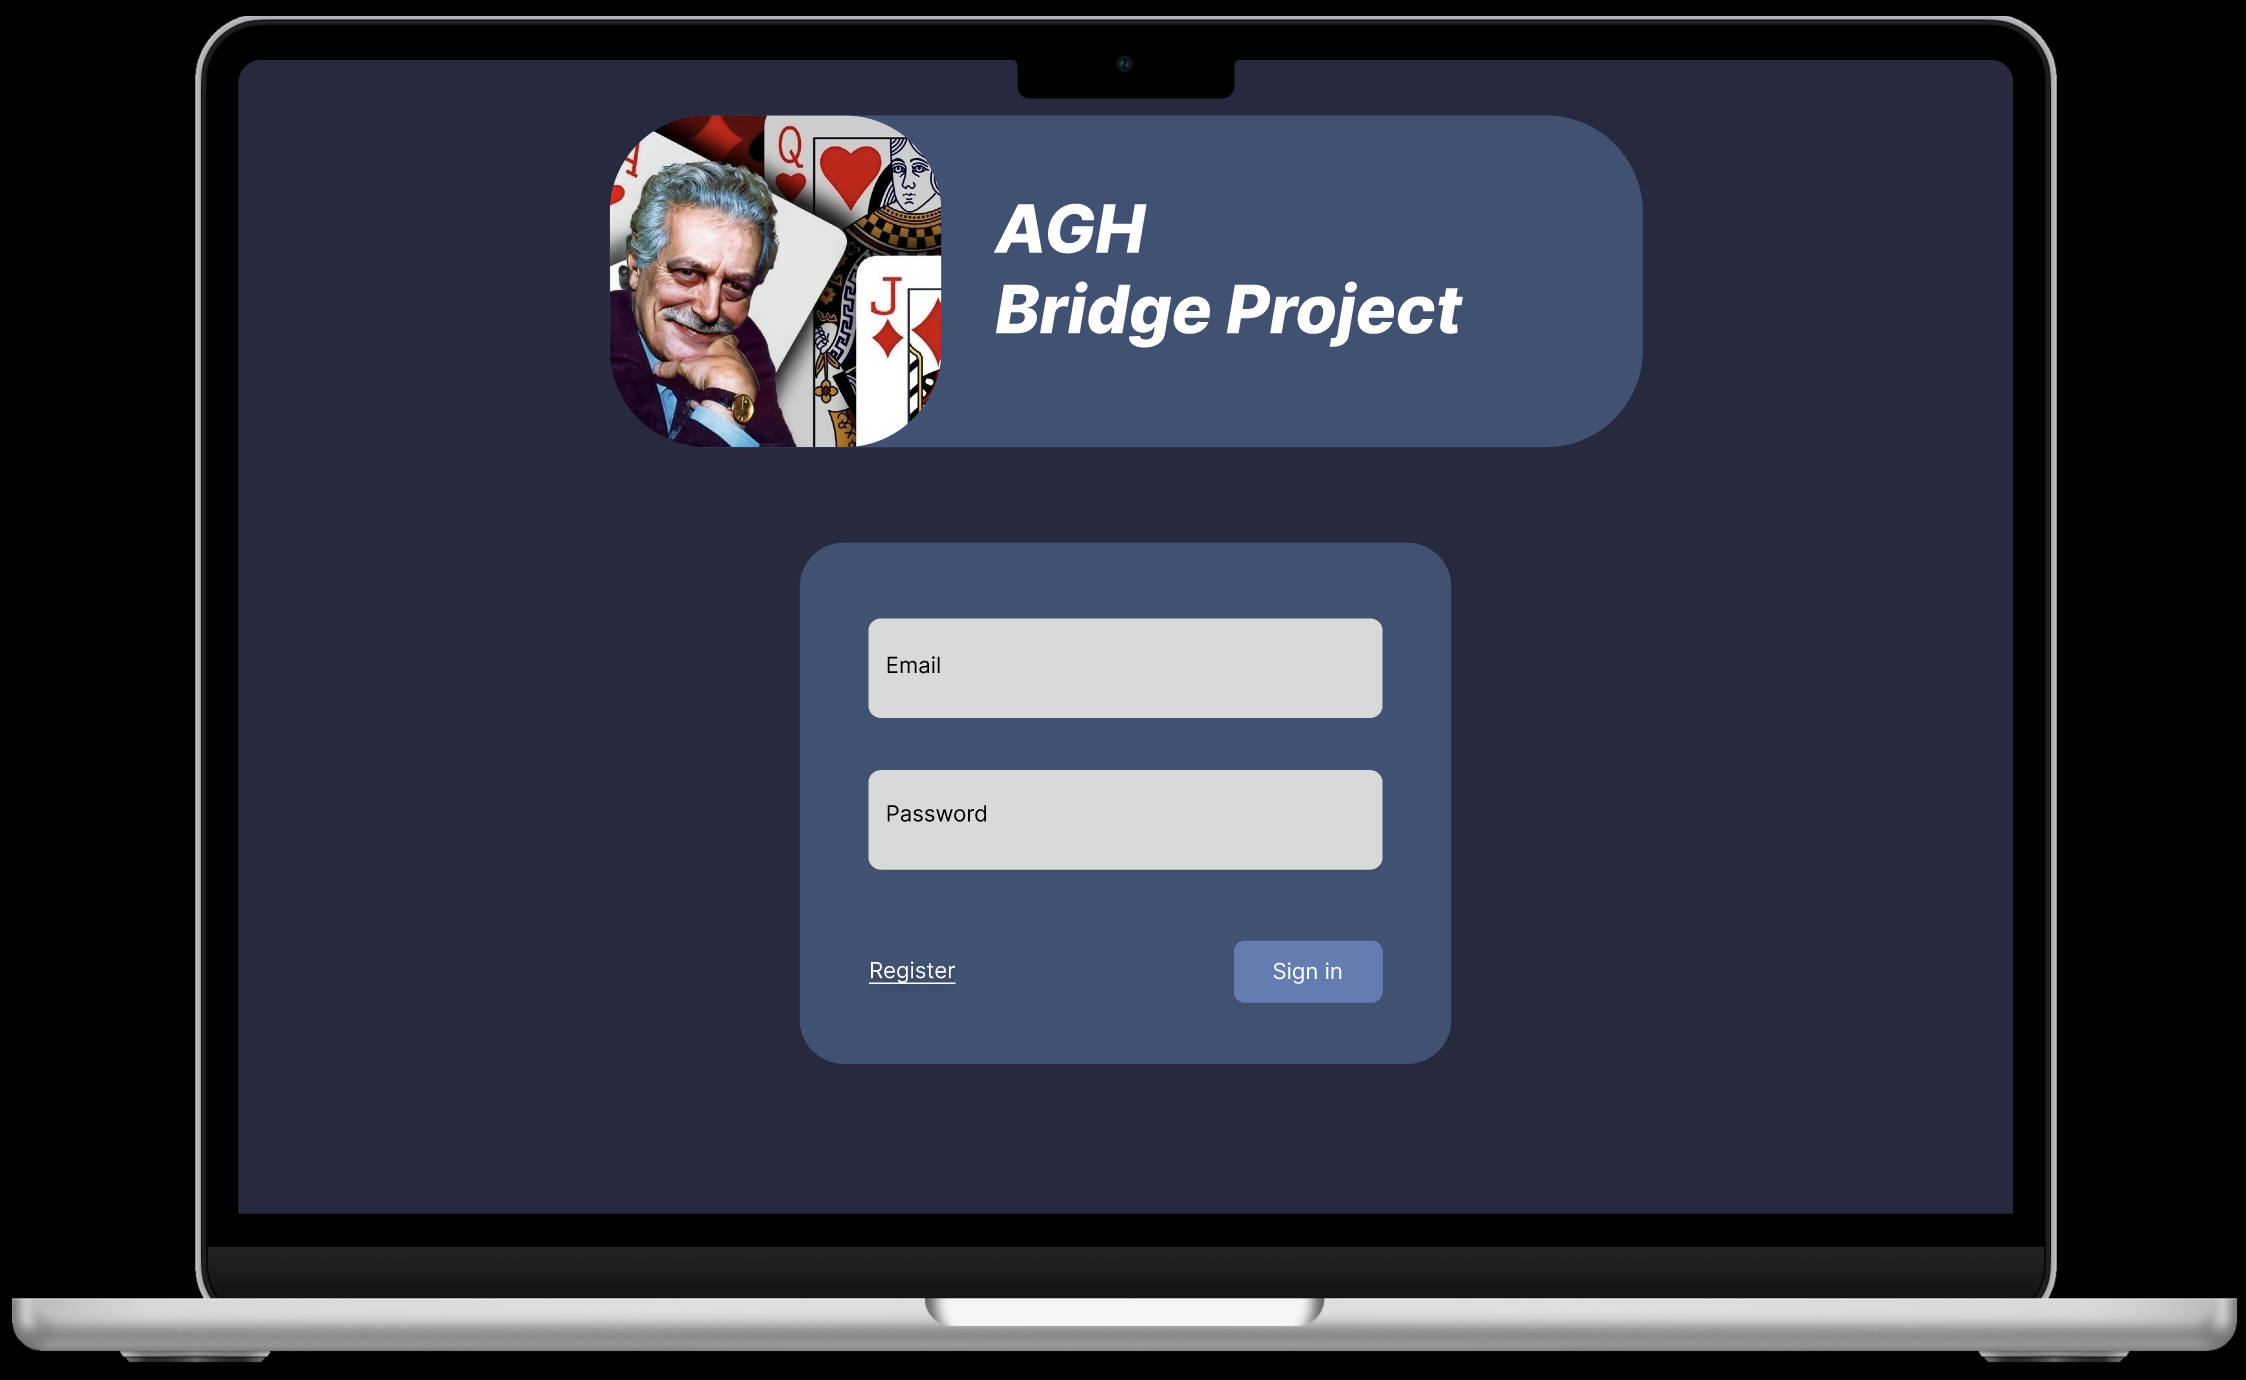
\includegraphics[width=0.45\textwidth]{img/figma-szkic/1.png}
        \label{fig:figma_login}
    }%
    \hspace*{0.5cm}
    \subfloat[Ekran główny]{
        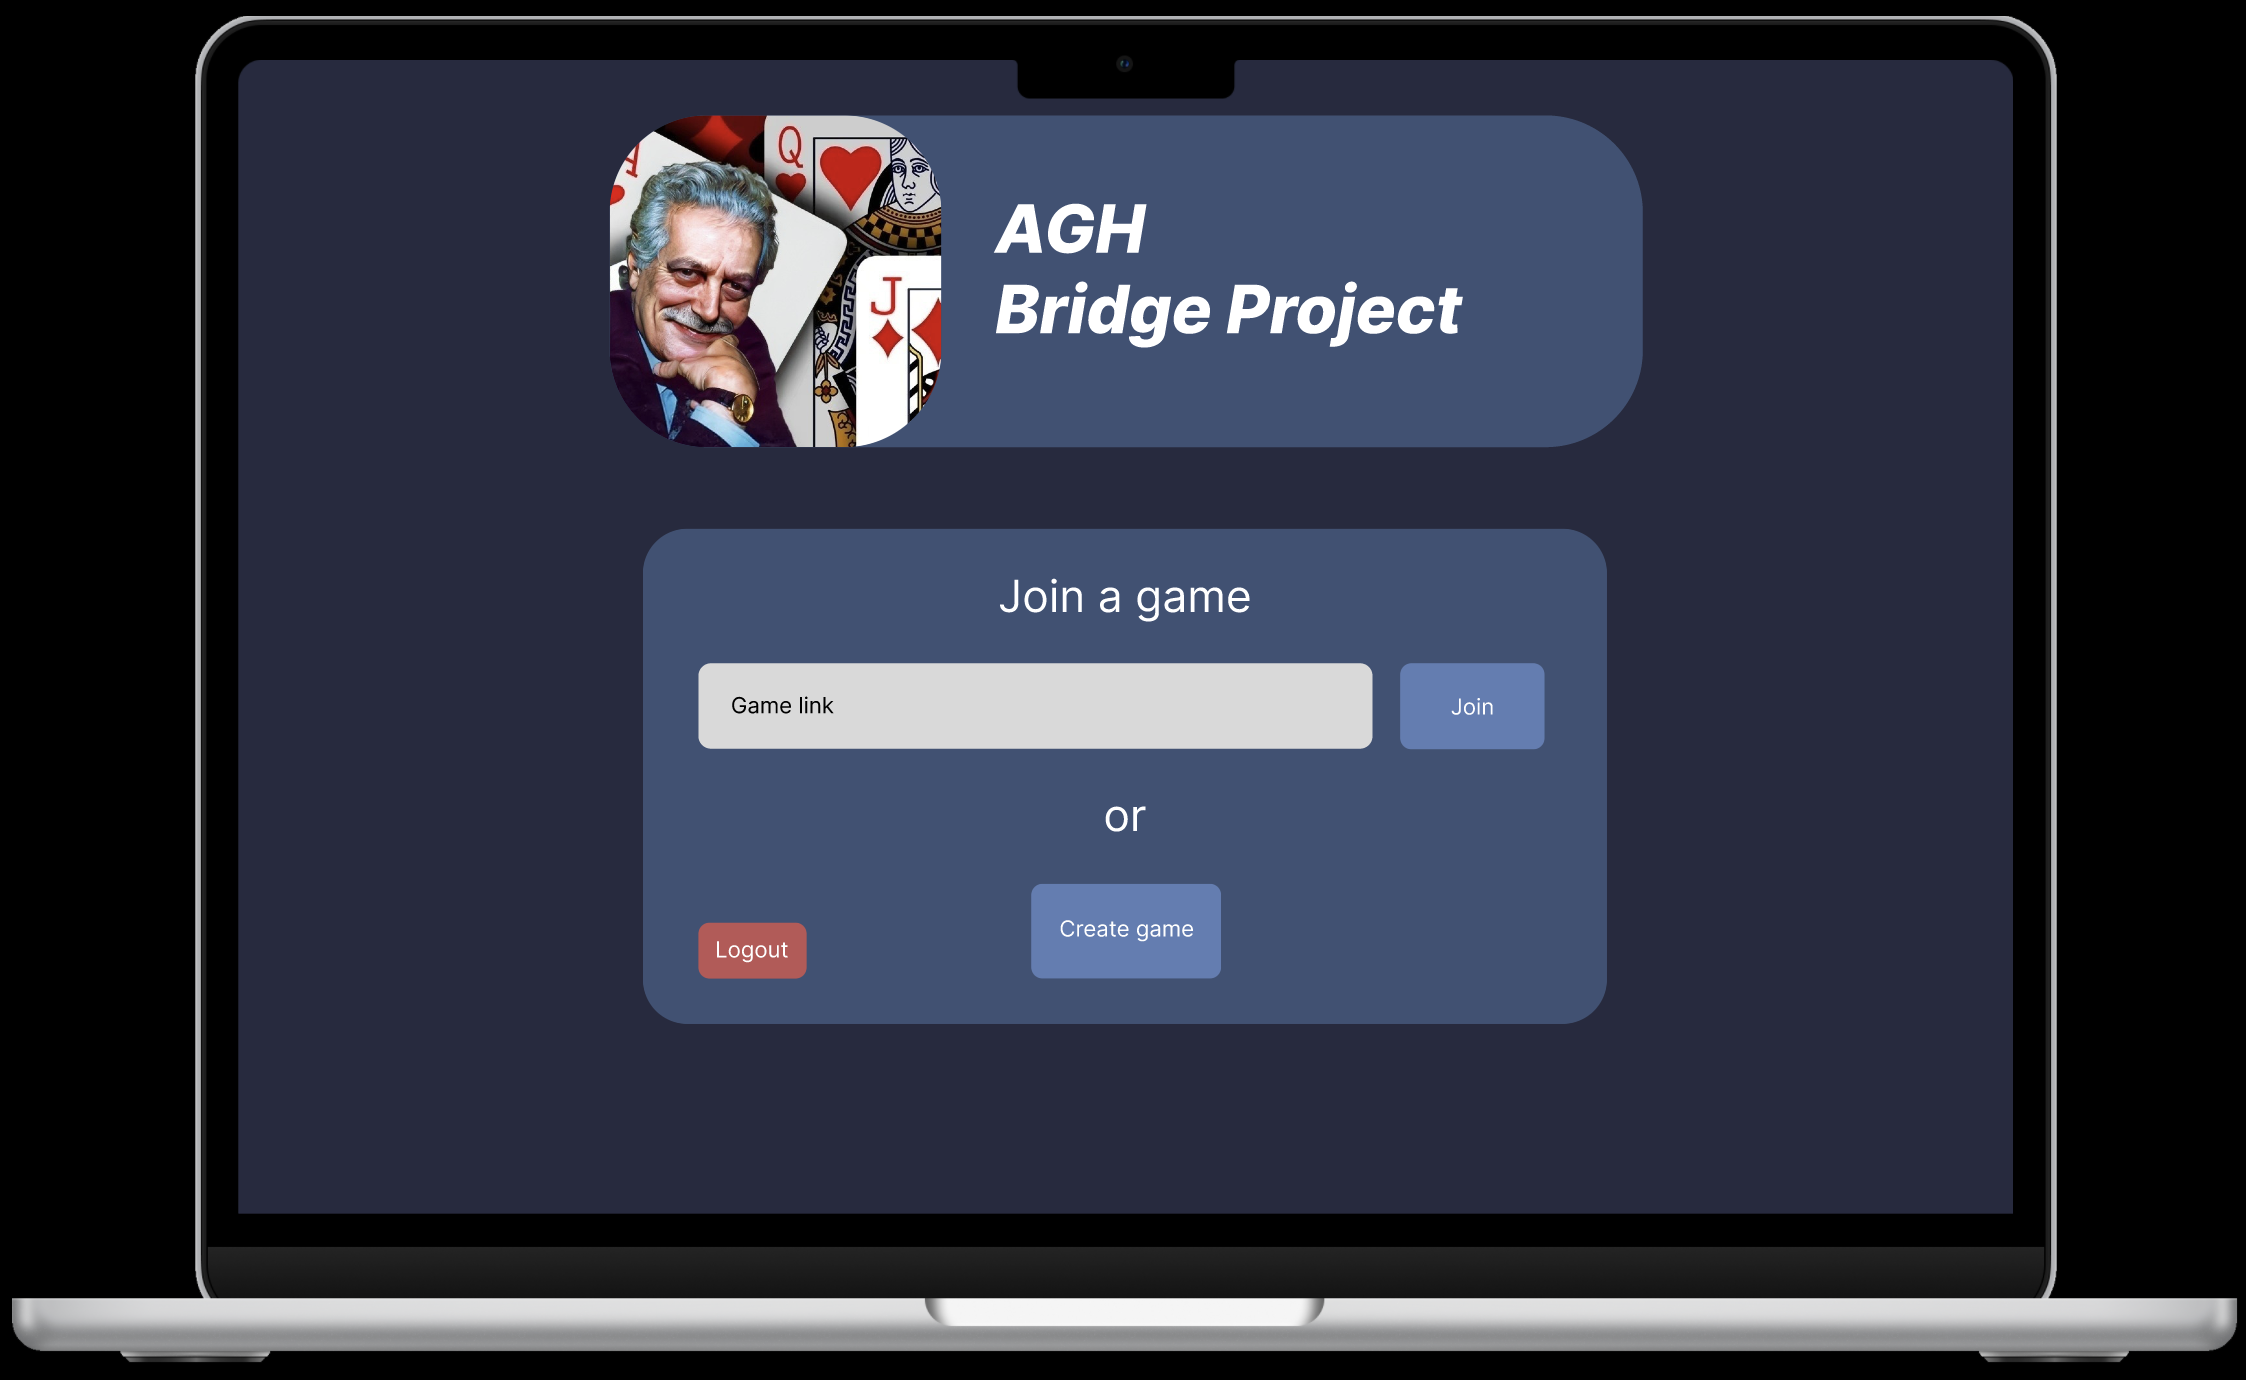
\includegraphics[width=0.45\textwidth]{img/figma-szkic/2.png}
    }%
    \\
    \subfloat[Ekran lobby]{
        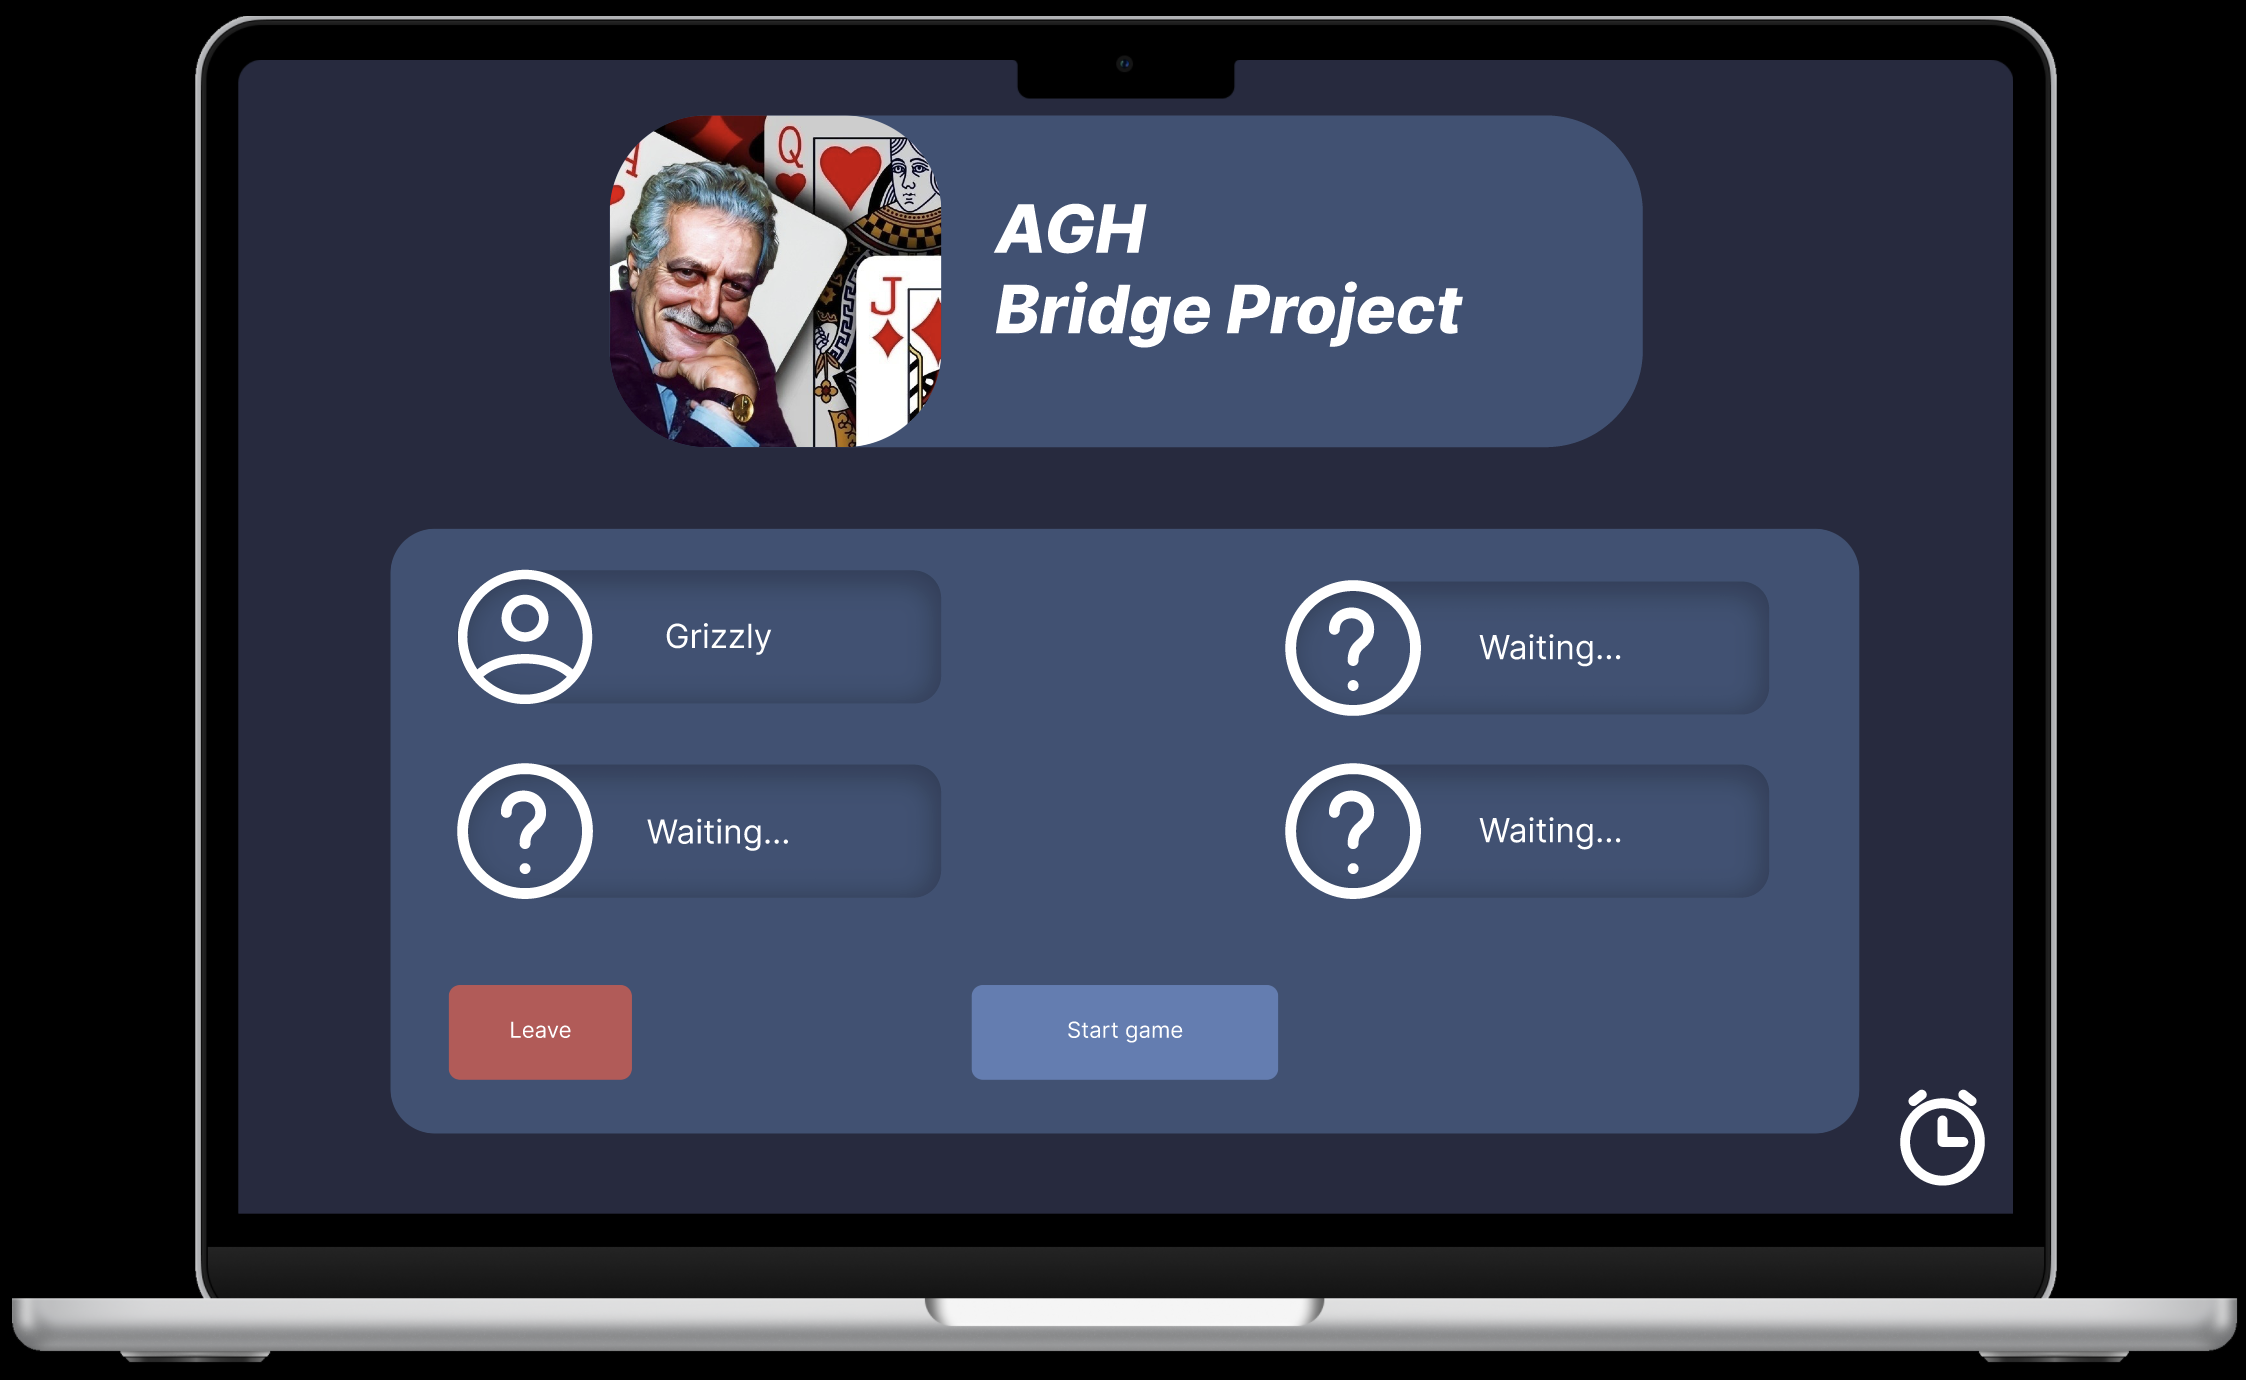
\includegraphics[width=0.45\textwidth]{img/figma-szkic/3.png}
    }%
    \hspace*{0.5cm}
    \subfloat[Ekran gry]{
        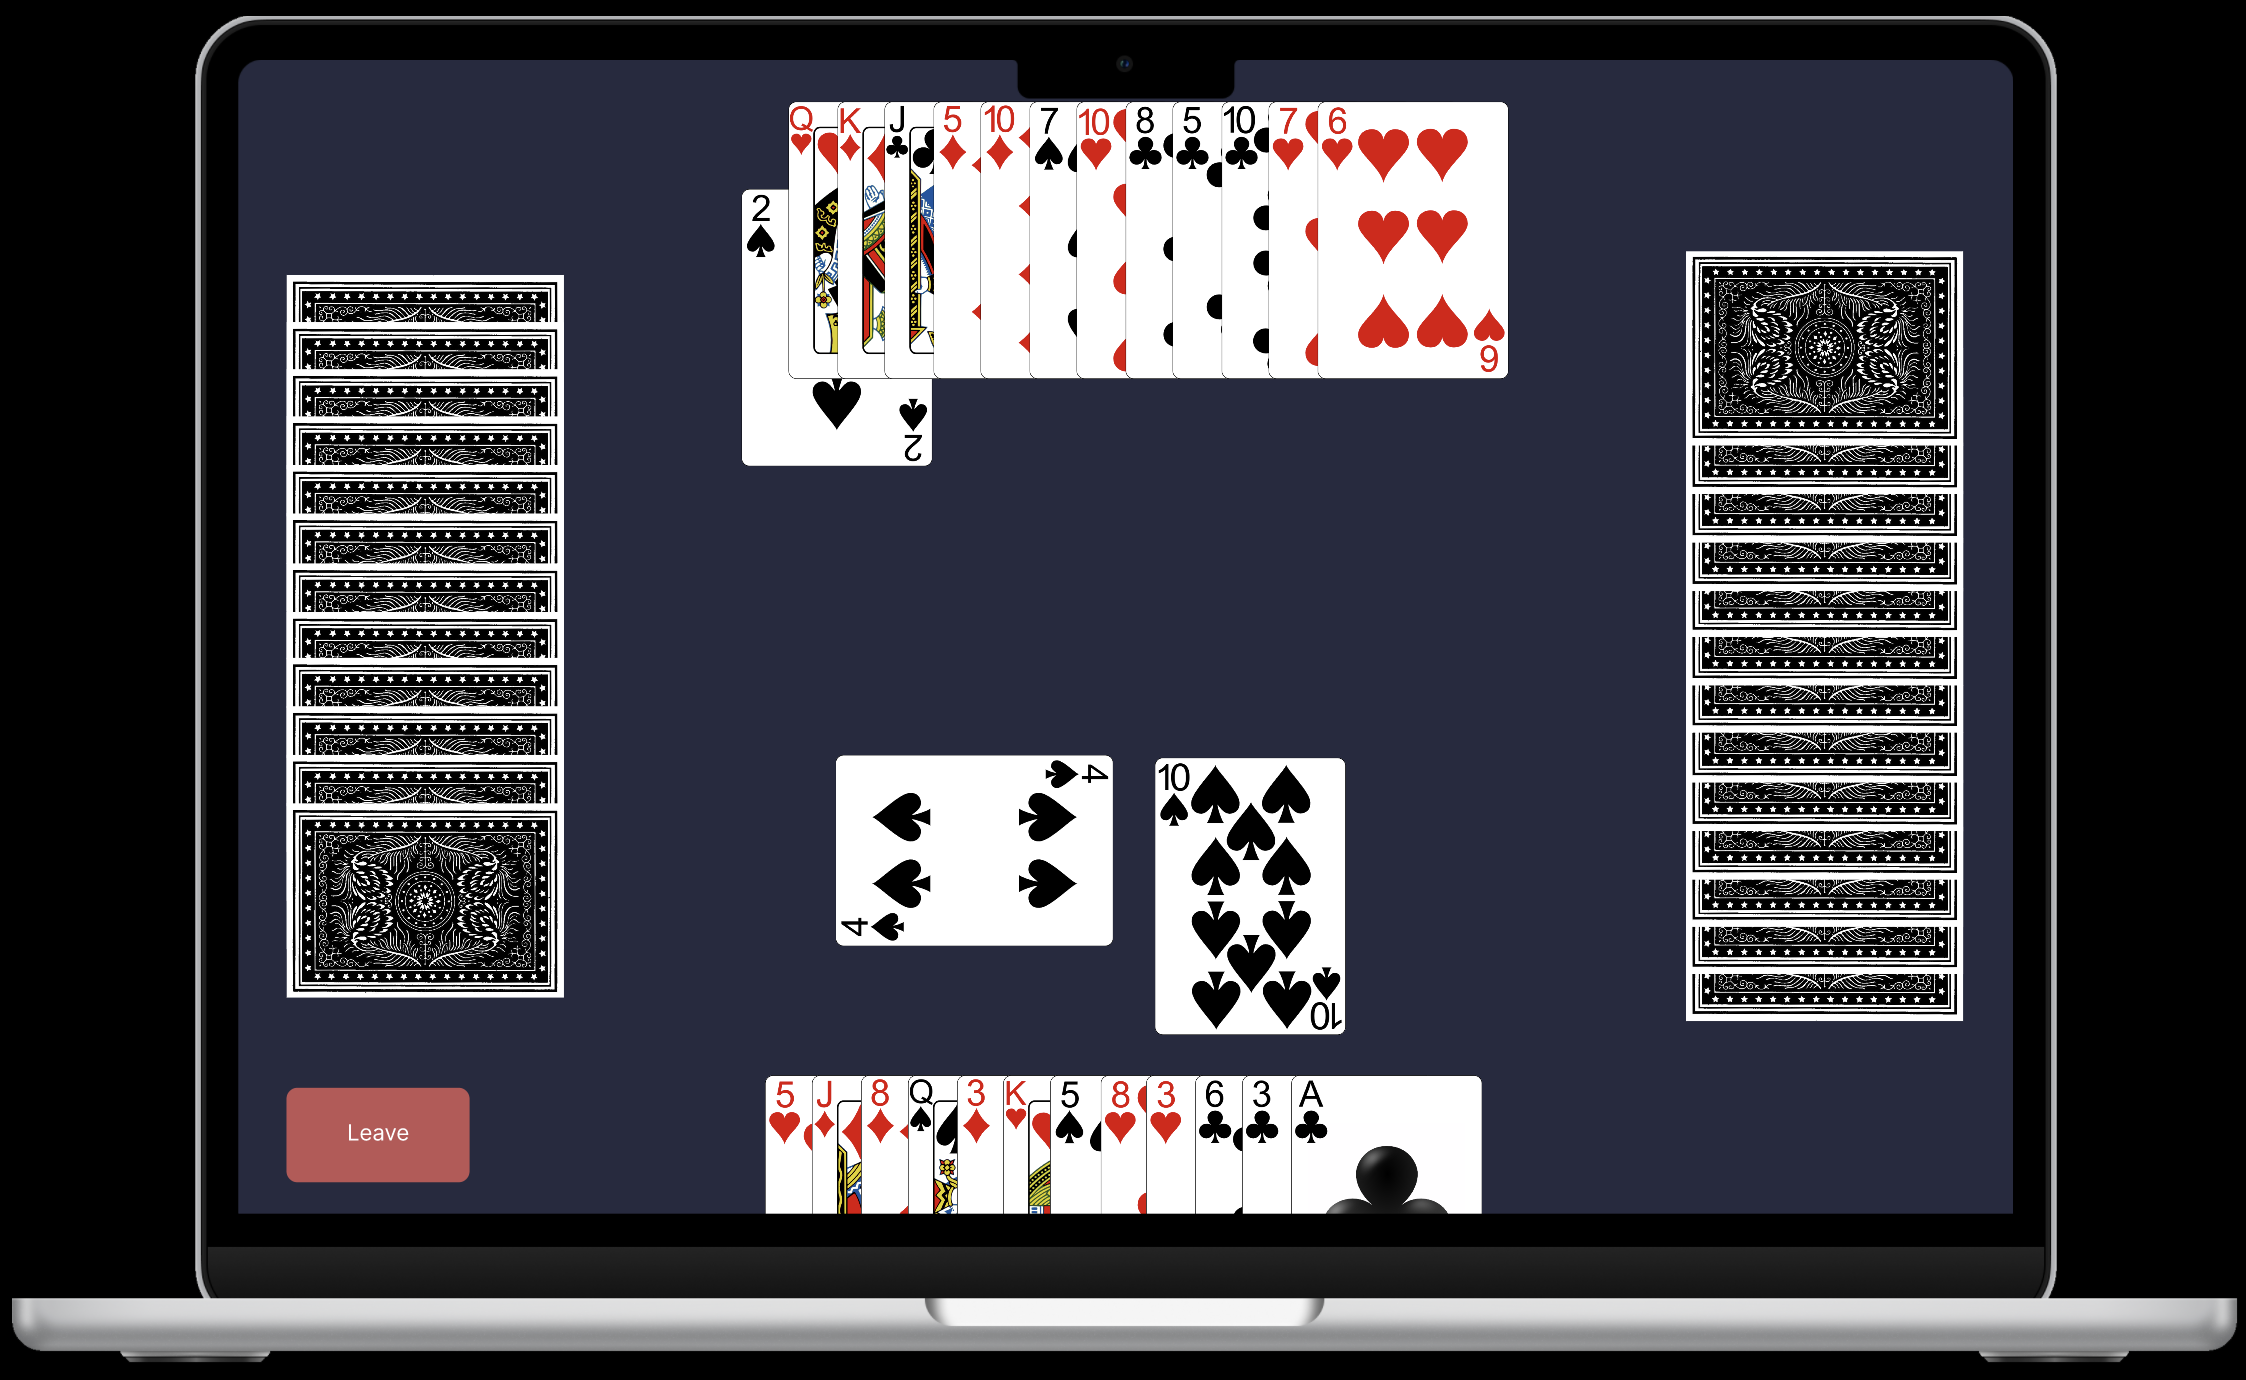
\includegraphics[width=0.45\textwidth]{img/figma-szkic/4.png}
        \label{fig:figma_game}
    }%
    \caption{Szkice interfejsu aplikacji}
\end{figure}

\FloatBarrier

\section{Słownik pojęć}

\begin{enumerate}
    \item Brydż -- karciana gra strategiczna rozgrywana przez dwie pary graczy,
    \item Użytkownik -- człowiek korzystający z aplikacji,
    \item Wirtualny asystent -- algorytm posiadający możliwość analizy rozgrywki w celu nauki, współpracy lub konkurencji z użytkownikiem,
    \item Gracz -- użytkownik lub wirtualny asystent biorący udział w rozgrywce,
    \item Partner -- drugi gracz grający w parze danego gracza,
    \item Przeciwnik -- jeden z graczy z pary grającej przeciwko danemu graczowi,
    \item Wirtualny partner -- partner będący wirtualnym asystentem,
    \item Wirtualny przeciwnik -- przeciwnik będący wirtualnym asystentem,
\end{enumerate}
